\documentclass{beamer}
\usepackage{amsmath}
\usepackage[utf8]{inputenc}
\usepackage{graphics}
\usepackage{hyperref}
\usepackage{xcolor}
\usepackage{wasysym}
\usepackage{listings}
\usepackage{tikz}
\usepackage{amssymb}
\usepackage[normalem]{ulem}
\usepackage{textcomp}
\usepackage{verbatim}
\usepackage[T1]{fontenc}
\usepackage{lmodern}
\usetikzlibrary{shapes.callouts,shadows, calc}

\tikzset{note/.style={rectangle callout, rounded corners,fill=gray!20,drop shadow,font=\footnotesize}}    
\newcommand{\tikzmark}[1]{\tikz[overlay,remember picture] \node (#1) {};}    

\newcounter{image}
\setcounter{image}{1}

\makeatletter
\newenvironment{btHighlight}[1][]
{\begingroup\tikzset{bt@Highlight@par/.style={#1}}\begin{lrbox}{\@tempboxa}}
{\end{lrbox}\bt@HL@box[bt@Highlight@par]{\@tempboxa}\endgroup}

\newcommand\btHL[1][]{%
  \begin{btHighlight}[#1]\bgroup\aftergroup\bt@HL@endenv%
}
\def\bt@HL@endenv{%
  \end{btHighlight}%   
  \egroup
}
\newcommand{\bt@HL@box}[2][]{%
  \tikz[#1]{%
    \pgfpathrectangle{\pgfpoint{0pt}{0pt}}{\pgfpoint{\wd #2}{\ht #2}}%
    \pgfusepath{use as bounding box}%
    \node[anchor=base west,rounded corners, fill=green!30,outer sep=0pt,inner xsep=0.2em, inner ysep=0.1em,  #1](a\theimage){\usebox{#2}};
  }%
 \stepcounter{image}
}
\makeatother

\usetheme{Warsaw}
\usecolortheme{lily}
\setbeamercovered{transparent}
\setbeamertemplate{headline}{
  \begin{beamercolorbox}{section in head/foot}
    \vskip2pt\insertnavigation{\paperwidth}\vskip2pt
  \end{beamercolorbox}
}

\setbeamertemplate{footline}{
}

\author{
  {\tiny Tony Morris\\}
}

\xdefinecolor{darkgreen}{rgb}{0,0.35,0}
\lstset{
  tabsize=2,
  basicstyle=\ttfamily,
  moredelim=**[is][\btHL]{`}{`}
}
\lstdefinestyle{java}{
  language=java,
  basicstyle=\footnotesize\ttfamily,
  stringstyle=\color{darkgreen}\ttfamily,
  commentstyle=\color{gray}\ttfamily,
  keywordstyle=\footnotesize\color{blue}\ttfamily,
  tabsize=2,
  moredelim=**[is][\btHL]{`}{`}
}
\lstdefinelanguage{scala}{
  morekeywords={abstract,case,catch,class,def,%
    do,else,extends,false,final,finally,%
    for,forSome,if,implicit,import,lazy,match,%
    new,null,object,override,package,%
    private,protected,requires,return,sealed,%
    super,this,throw,trait,true,try,%
    type,val,var,while,with,yield},
  otherkeywords={=,=>,<-,<\%,<:,>:,\#,@},
  sensitive=true,
  morecomment=[l]{//},
  morecomment=[n]{/*}{*/},
  morestring=[b]",
  morestring=[b]',
  morestring=[b]"""
}
\lstdefinelanguage{haskell}{
  morekeywords={class,instance,where,do,data,newtype,default,deriving,module},
  otherkeywords={<-},
  sensitive=true,
  morecomment=[l]{--},
  morecomment=[n]{\{-}{-\}}, 
  morestring=[b]",
  morestring=[b]',
  morestring=[b]"""
}
\lstdefinestyle{scala}{
  language=scala,
  basicstyle=\footnotesize\ttfamily,
  stringstyle=\color{darkgreen}\ttfamily,
  commentstyle=\color{gray}\ttfamily,
  keywordstyle=\footnotesize\color{blue}\ttfamily,
  tabsize=2,
  moredelim=**[is][\btHL]{`}{`}
}
\lstdefinestyle{haskell}{
  language=haskell,
  basicstyle=\tiny\ttfamily,
  stringstyle=\color{darkgreen}\ttfamily,
  commentstyle=\color{gray}\ttfamily,
  keywordstyle=\tiny\color{blue}\ttfamily,
  tabsize=2
}
% #866eaa
\definecolor{nicta-purple}{rgb}{0.5234,0.4297,0.6640}

\defbeamertemplate*{title page}{customized}[1][] {
  \centering
  \color{nicta-purple}
  \usebeamerfont{title}\inserttitle\par
  \bigskip
  \usebeamerfont{subtitle}\insertsubtitle\par
  \bigskip
  \bigskip
  \bigskip
  \bigskip
  \usebeamerfont{institute}\insertinstitute\par
  \bigskip
  \usebeamerfont{author}\insertauthor\par
  % \usebeamerfont{date}\insertdate\par
  \usebeamercolor[fg]{titlegraphic}\inserttitlegraphic
}

\logo{
\includegraphics[height=0.8cm]{image/nicta.jpg}}

\begin{document}
\title{\large Parametricity}
\subtitle{\small Types Are Documentation}
\institute[NICTA]{}
\tiny{\date

}
\normalsize

\setbeamercovered{transparent}
\begin{frame}
  \titlepage
\end{frame}

\begin{frame}
\frametitle{The Journey}
\framesubtitle{Fast and loose reasoning is morally correct}

\begin{block}{Danielsson, Hughes, Jansson \& Gibbons \cite{danielsson2006fast} tell us:}
\begin{quotation}
Functional programmers often reason about programs as if
they were written in a total language, expecting the results
to carry over to non-total (partial) languages. We justify
such reasoning.
\end{quotation}
\end{block}
\end{frame}

\begin{frame}
\frametitle{The Journey}
\framesubtitle{Theorems for Free!}
\begin{block}{Philip Wadler \cite{wadler1989theorems} tells us:}
\begin{quotation}
Write down the definition of a polymorphic function on a piece of paper. Tell me its type, but be careful not to let me see the function's definition. I will tell you a theorem that the function satisfies.

The purpose of this paper is to explain the trick.
\end{quotation}
\end{block}

\end{frame}

\begin{frame}
\frametitle{Scala}
\begin{itemize}
  \item We will use the Scala programming language for code examples
  \item However, nothing in this talk relates to Scala specifically
\end{itemize}
\end{frame}

\begin{frame}
\frametitle{Scala}
\begin{center}
However, other languages may be used syntax to denote important concepts and ensure clarity.
\end{center}
\begin{center}

\includegraphics[height=1.8cm]{image/tissues.jpg}
\end{center}
\end{frame}

\begin{frame}
\frametitle{Why Scala?}
\begin{itemize}
  \item Scala is a legacy programming language
  \item Yet it is capable of achieving a high degree of code reasoning
  \item Please speak up if unfamiliarity of syntax inhibits understanding
\end{itemize}
\end{frame}

\begin{frame}
\frametitle{Yeah so?}
\begin{itemize}
  \item In other words, we can still shoot high, even with inferior systems like Scala
  \item A lot of Scala users are noisy about code readability and say awesome (i.e. some awe) things on the matter
  \item<2-> I have a special place in my heart for this kind of confusion $\heartsuit$
\end{itemize}
\end{frame}

\begin{frame}[fragile]
\frametitle{Lossful Reasoning}
\framesubtitle{Sacrificing efficiency to gain unreliability}
Suppose we encountered the following function definition:
\begin{lstlisting}[style=scala]
def add10(n: Int): Int
\end{lstlisting}
By the type alone, there are {$({2^{32}})^{2^{32}}$} possible implementations.
\end{frame}

\begin{frame}[fragile]
\frametitle{Lossful Reasoning}
\framesubtitle{Sacrificing efficiency to gain unreliability}
We might form a suspicion that \lstinline[style=scala]$add10$ adds ten to its argument.
\begin{lstlisting}[style=scala]
def `add10`(n: Int): Int
\end{lstlisting}
\begin{tikzpicture}[remember picture,overlay]
\coordinate (aa) at ($(a1)+(7,2.0)$);
\node[note,draw,callout relative pointer={($(aa)-(11.2,-3.7)$)},right] at (aa) {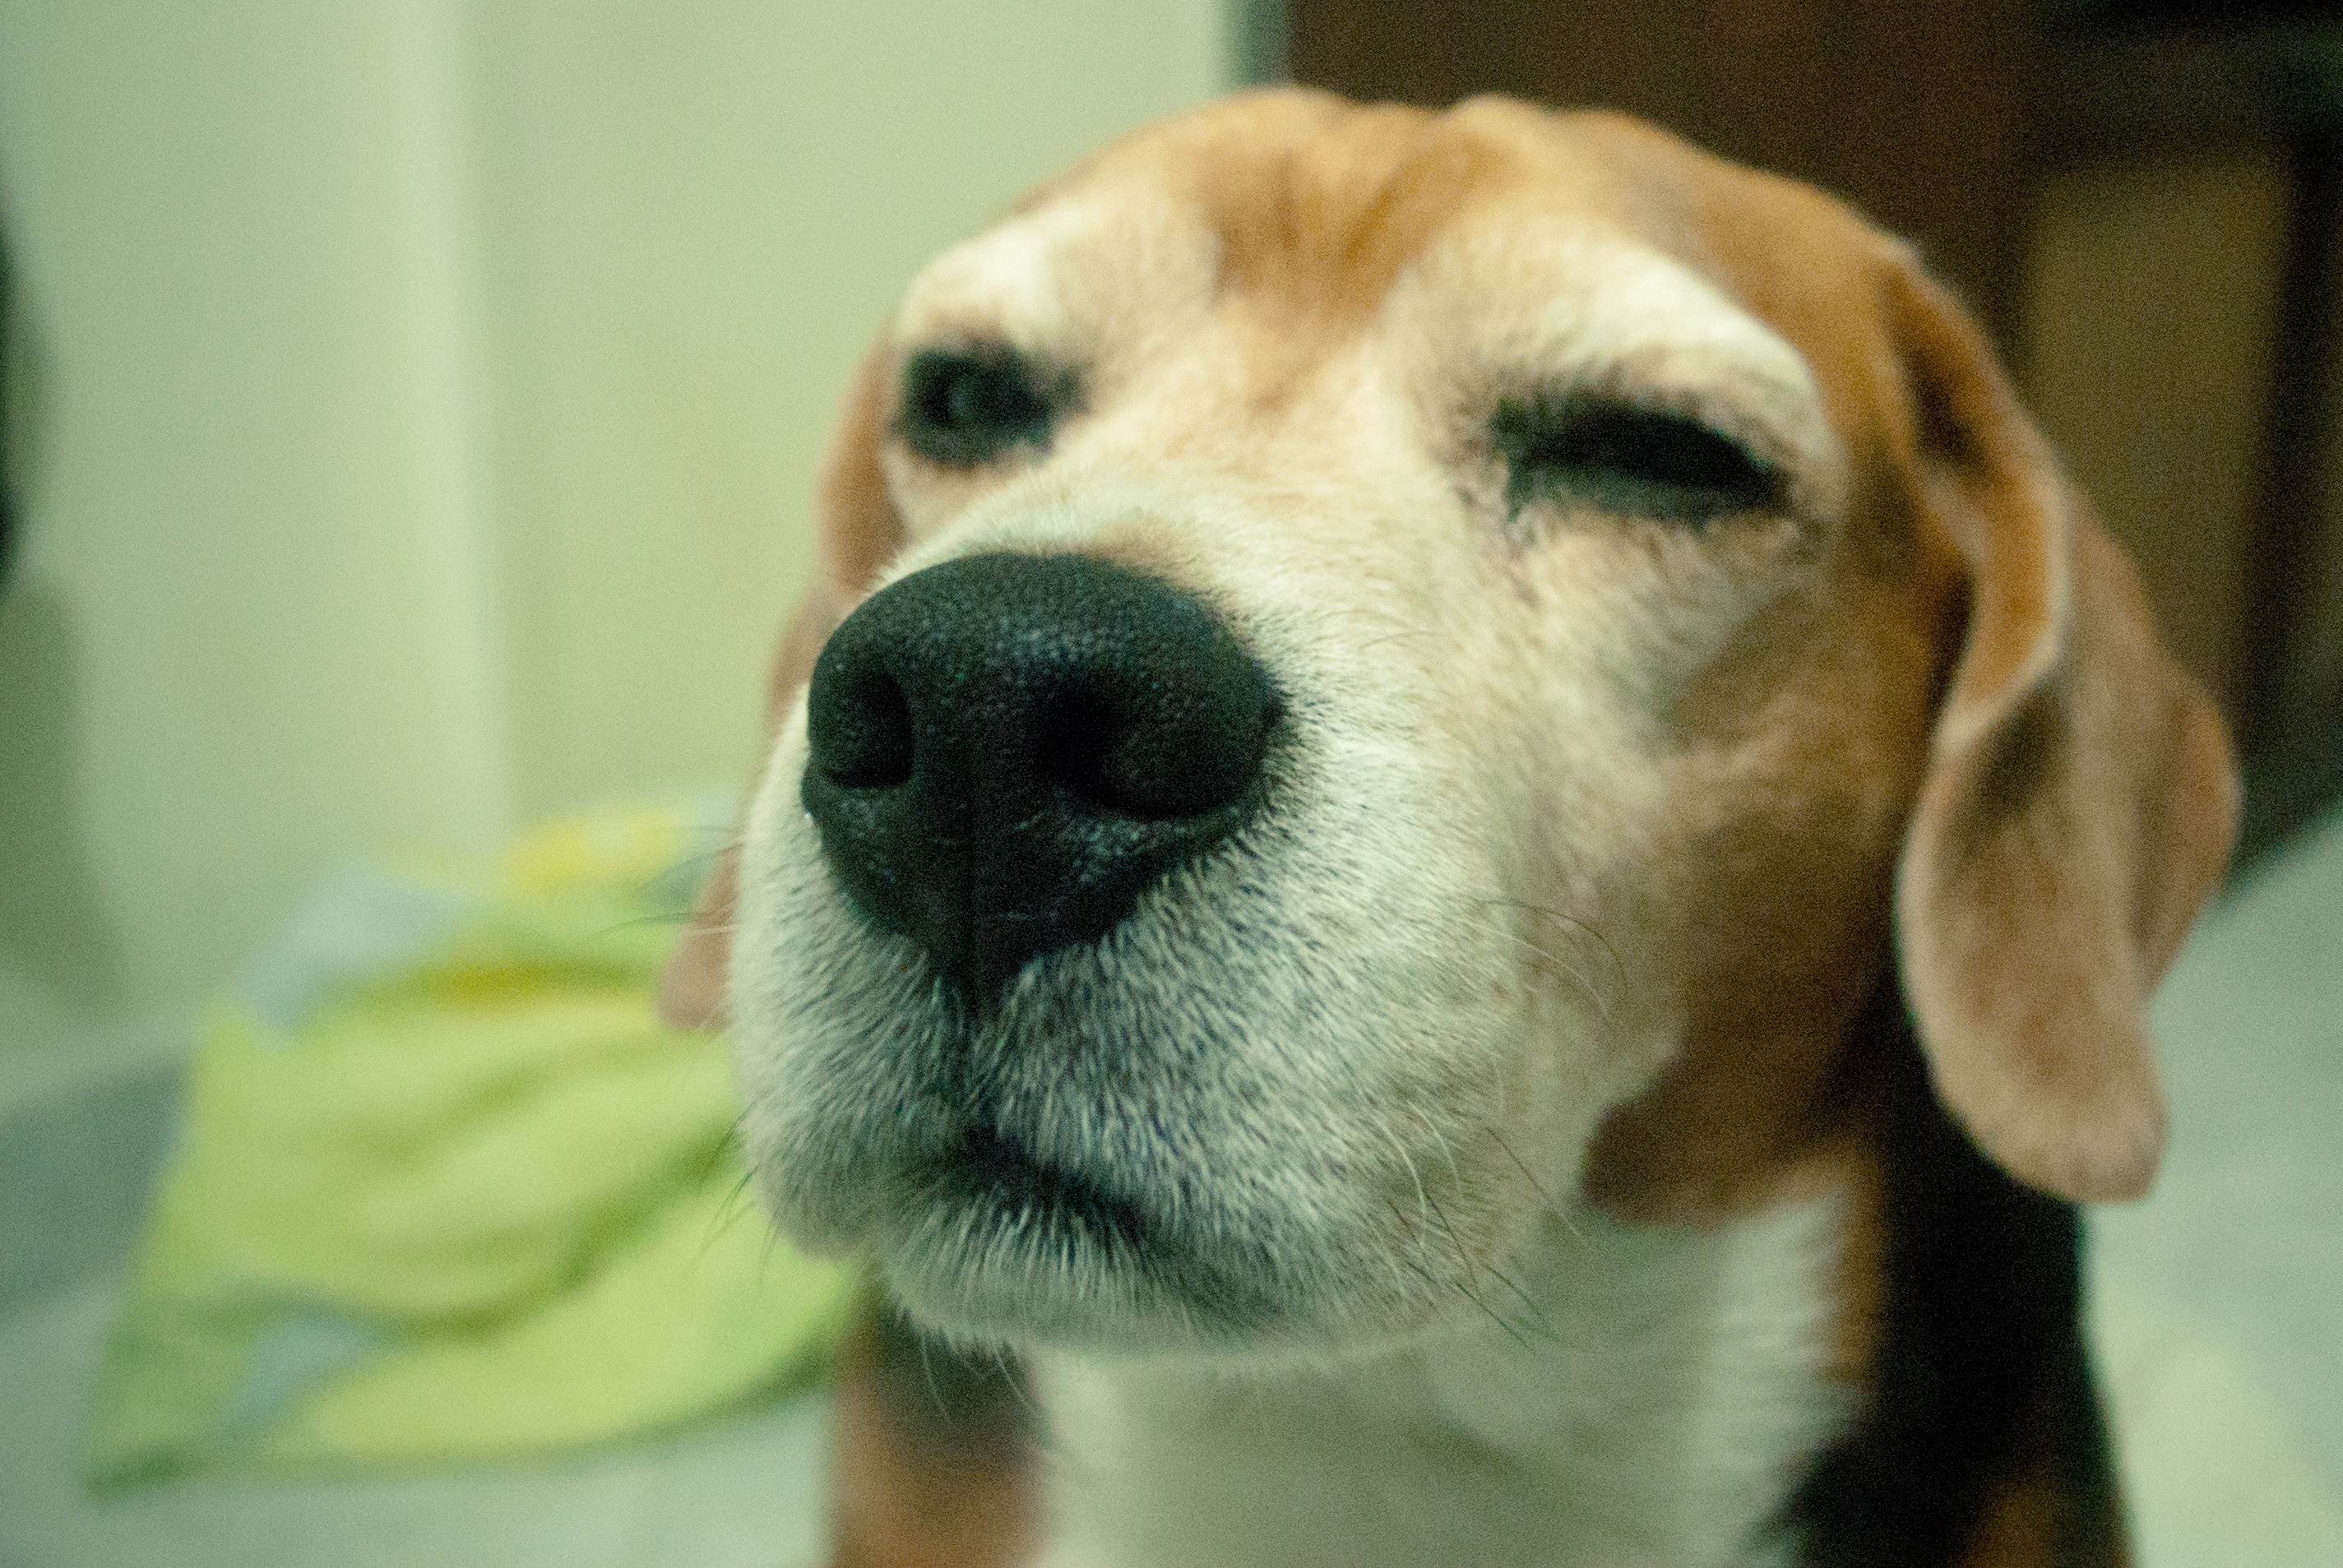
\includegraphics[width=0.2\textwidth]{image/suspicion.jpg}};
\end{tikzpicture}
\end{frame}

\begin{frame}[fragile]
\frametitle{Lossful Reasoning}
\framesubtitle{Sacrificing efficiency to gain unreliability}
So we write some tests:
\begin{lstlisting}[style=scala]
add10(0)        = 10
add10(5)        = 15
add10(-5)       = 5
add10(223)      = 233
add10(5096)     = 5106
add10(2914578)  = 29145588
add10(-2914578) = -29145568
\end{lstlisting}
And conclude, yes, this function adds ten to its argument.
\end{frame}

\begin{frame}[fragile]
\frametitle{Lossful Reasoning}
\framesubtitle{Sacrificing efficiency to gain unreliability}
We have just failed the Wason Rule Discovery Test.
\begin{lstlisting}[style=scala]
def add10(n: Int): Int =
  if(n < 8000000) n + 10
  else n * 7
\end{lstlisting}
This is due to a \emph{confirmation bias\cite{gale2002does}}.
\end{frame}

\begin{frame}[fragile]
\frametitle{Lossful Reasoning}
\framesubtitle{Sacrificing efficiency to gain unreliability}
We will just write more tests!
\begin{lstlisting}[style=scala]
add10(18916712)  = 18916722
add10(-18916712) = -18916702
\end{lstlisting}
\ldots or we might come up with some system of apologetics for this shortfall.
\begin{itemize}
  \item ``A negligent programmer has misnamed this function"
  \item ``More tests will fix it"
  \item ``Well we can't test everything!"
\end{itemize}
\end{frame}

\begin{frame}[fragile]
\frametitle{Lossful Reasoning}
\framesubtitle{Sacrificing efficiency to gain unreliability}
\begin{center}{We are simply reinforcing the confirmation bias by strengthening 
the excess confidence in our belief that we are being responsible programmers.}
\end{center}
\end{frame}

\begin{frame}[fragile]
\frametitle{Lossful Reasoning}
\framesubtitle{Sacrificing efficiency to gain unreliability}
\begin{center}
We aren't.
\end{center}
\end{frame}

\begin{frame}[fragile]
\frametitle{Lossful Reasoning}
\framesubtitle{Sacrificing efficiency to gain unreliability}
\begin{block}{But\ldots}
there are {$({2^{32}})^{2^{32}}$} possible implementations. Surely we cannot 
rule out the existence of \emph{all-but-one} of those? We can only rule out a
\scriptsize{very, very} \tiny{small subset}!
\end{block}
\end{frame}

\begin{frame}[fragile]
\frametitle{Lossful Reasoning}
\framesubtitle{Efficiency}
\begin{center}
Actually, we can.
\end{center}
\end{frame}

\begin{frame}[fragile]
\frametitle{Lossful Reasoning}
\framesubtitle{Reliability}
\begin{center}
And we can have a machine-checked proof, mitigating our disposition to
confirmation bias.
\end{center}
\end{frame}

\begin{frame}[fragile]
\frametitle{Reasoning with parametricity}
\begin{block}{Monomorphic Signature}
\begin{itemize}
  \item Examining the signature \lstinline[style=scala]{Int => Int}
  \item We see a lot of things this function does \emph{not} do
  \item For example, it never returns \lstinline[style=scala]{"abc"}
  \item However, there is an unmanageable number of possible things it might do
\end{itemize}
\end{block}
\end{frame}

\begin{frame}[fragile]
\frametitle{Reasoning with parametricity}
\begin{block}{Another monomorphic example}
\begin{itemize}
  \item Examining the signature \lstinline[style=scala]{List[Int] => List[Int]}
  \item For example, it might add all the \lstinline{Int}s and return a list arrangement that depends on whether or not the result is a prime number
  \item The possibilities are \emph{enormous}
\end{itemize}
\end{block}
\end{frame}

\begin{frame}[fragile]
\frametitle{Reasoning with parametricity}
\begin{block}{Parametric Signature}
\begin{lstlisting}[style=scala]
def `irrelevant`[A](x: List[A]): List[A]
\end{lstlisting}
\begin{itemize}
  \item We can immediately assert, with confidence, a lot of things about how this function works \emph{because it is parametric\footnote{or polymorphic}}
  \item More directly, we assert what the function does not do
  \item<2> In other words, \emph{parametricity} has improved readability
  \item<2> Really? By how much?
\end{itemize}
\end{block}
\end{frame}

\begin{frame}[fragile]
\frametitle{Reasoning with parametricity}
\begin{lstlisting}[style=scala]
def `irrelevant`[A](x: List[A]): List[A] = 
  ...
\end{lstlisting}
\begin{theorem}Every element \lstinline{A} in the result list appears in the input. Contraposed, If \lstinline{A} is not in the input, it is not in the result\end{theorem}
\end{frame}

\begin{frame}[fragile]
\frametitle{Reasoning with parametricity}
\begin{block}{I know this because \ldots}
\begin{itemize}
  \item<1> Because I am the boss and I said so
  \item<2> Because Reliable Rob told me so
  \item<3> Because the \emph{function name} told me so
  \item<4> Because the comment told me so
  \item<5> \textbf{Because it would not have compiled otherwise}
\end{itemize}
\end{block}
\end{frame}

\begin{frame}[fragile]
\frametitle{Reasoning with parametricity}
\begin{block}{Another example}
\begin{lstlisting}[style=scala]
def reverse[A, B](x: List[A]): List[B] = 
  ...
\end{lstlisting}
\end{block}
\begin{theorem}This function reverses the input list, because the name says so\end{theorem}
\end{frame}

\begin{frame}[fragile]
\frametitle{Reasoning with parametricity}
\begin{block}{Lies}
\begin{lstlisting}[style=scala]
def reverse[A, B](x: List[A]): List[B] = 
  ...
\end{lstlisting}
\end{block}
\begin{theorem}This function \textbf{always} returns \lstinline{Nil} otherwise it would not have compiled\end{theorem}
\end{frame}

\begin{frame}[fragile]
\frametitle{Reasoning with parametricity}
\begin{block}{Uninhabited Example}
\begin{lstlisting}[style=scala]
def irrelevant[A, B](a: A): B = 
  ...
\end{lstlisting}
\end{block}
\begin{theorem}This function \textbf{never} returns because it will never compile\end{theorem}
\end{frame}

\begin{frame}[fragile]
\frametitle{Reasoning with parametricity}
\begin{block}{Fast and loose reasoning is morally correct \cite{danielsson2006fast}}
\small{Functional programmers often reason about programs as if
they were written in a total language, expecting the results
to carry over to non-total (partial) languages. We justify
such reasoning.}
\end{block}
What does this mean exactly?
\end{frame}

\begin{frame}[fragile]
\frametitle{Fast and Loose Reasoning}
\begin{fact}Non-totality is a consequence of any turing-complete system\end{fact}
\end{frame}

\begin{frame}[fragile]
\frametitle{Fast and Loose Reasoning}
\begin{itemize}
  \item This means that any turing-complete system will permit \emph{escape hatches for partiality}.
  \item Each turing-complete system has different, specialised mechanisms that permit partiality.
  \item These escape hatches undermine the value of our assertions \ldots but let's not throw away everything.
\end{itemize}
\end{frame}

\begin{frame}[fragile]
\frametitle{Fast and Loose Reasoning}
\begin{block}{Scala has a few escape hatches}
\begin{itemize}
  \item \lstinline{null}
  \item exceptions
  \item Type-casing (\lstinline{isInstanceOf})
  \item Type-casting (\lstinline{asInstanceOf})
  \item Side-effects
  \item \lstinline{equals}/\lstinline{toString}/\lstinline{hashCode}
  \item \lstinline{notify}/\lstinline{wait}
  \item \lstinline{classOf}/\lstinline{.getClass}
  \item General recursion
\end{itemize}
\end{block}
\end{frame}

\begin{frame}[fragile]
\frametitle{Fast and Loose Reasoning}
\framesubtitle{\lstinline{null} escape hatch}
\begin{lstlisting}[style=scala]
def `irrelevant`[A](x: List[A]): List[A] = 
  null
\end{lstlisting}
\begin{theorem}Every \lstinline{A} element in the result list appears in the input list\end{theorem}
Well, not if you don't even have a list.
\end{frame}

\begin{frame}[fragile]
\frametitle{Fast and Loose Reasoning}
\framesubtitle{\lstinline{type-casing} escape hatch}
\begin{lstlisting}[style=scala]
def `irrelevant`[A](x: A): Boolean = 
  if(x.isInstanceOf[Int])
  else x match {
    case (s: String) => s.length < 10
  }
\end{lstlisting}
\begin{theorem}This function ignores its argument and consistently returns either \lstinline{true} or \lstinline{false}\end{theorem}
Type-casing\footnote{case-analysis on type} breaks parametricity and so undermines our theorems.
\end{frame}

\begin{frame}[fragile]
\frametitle{Fast and Loose Reasoning}
\framesubtitle{\lstinline{type-casting} escape hatch}
\begin{lstlisting}[style=scala]
def `irrelevant`[A](x: List[A]): List[A] = 
  "abc".asInstanceOf[A] :: x  
\end{lstlisting}
\begin{theorem}Every \lstinline{A} element in the result list appears in the input list\end{theorem}
\end{frame}

\begin{frame}[fragile]
\frametitle{Fast and Loose Reasoning}
\framesubtitle{\lstinline{side-effect} escape hatch}
\begin{lstlisting}[style=scala]
def `irrelevant`[A](x: A): A = {
    println("hi")
    x
  }
\end{lstlisting}
\begin{theorem}This function only ever does one thing \textemdash return its argument \end{theorem}
\end{frame}

\begin{frame}[fragile]
\frametitle{Fast and Loose Reasoning}
\framesubtitle{\lstinline{toString} escape hatch}
\begin{lstlisting}[style=scala]
def `irrelevant`[A](x: A): Int =
  x.toString.length
\end{lstlisting}
\begin{theorem}This function ignores its argument to return one of {${2^{32}}$} values. \end{theorem}
\end{frame}

\begin{frame}[fragile]
\frametitle{Fast and Loose Reasoning}
\framesubtitle{where to place our trust?}
\begin{lstlisting}[style=scala]
def reverse[A, B](x: List[A]): List[B] = 
  x.foldLeft[List[B]](Nil)((b, a) =>
    a.`asInstanceOf`[B] :: b)
\end{lstlisting}
\begin{theorem}This function \textbf{always} returns \lstinline{Nil} and so cannot possibly reverse the list\end{theorem}
\end{frame}

\begin{frame}[fragile]
\frametitle{Fast and Loose Reasoning}
\begin{itemize}
  \item Scala sure does have a lot of escape hatches!
  \item to what extent do they pervade our reasoning abilities?
  \item let us reframe the question
  \item if we abandon all these escape hatches, to what extent is the programming environment disabled?
\end{itemize}
\end{frame}

\begin{frame}[fragile]
\frametitle{Fast and Loose Reasoning}
\begin{itemize}
  \item Haskell disables side-effects, type-casing and type-casting, \emph{obtaining a total, relative advantage}.
  \item Agda goes further by disabling non-termination, again to its advantage.
  \item so what about Scala?
  \item can we use a reliable subset without too much penalty?
\end{itemize}
\end{frame}

\begin{frame}[fragile]
\frametitle{Fast and Loose Reasoning}
\frametitle{Safe Scala subset}
\begin{center}
Yes.
\end{center}
\begin{center}
And we do.
\end{center}
\end{frame}

\begin{frame}[fragile]
\frametitle{Fast and Loose Reasoning}
\begin{block}{Safe Scala subset}
\begin{itemize}
  \item \sout{\lstinline{null}}
  \item \sout{exceptions}
  \item \sout{Type-casing (\lstinline{isInstanceOf})}
  \item \sout{Type-casting (\lstinline{asInstanceOf})}
  \item \sout{Side-effects}
  \item \sout{\lstinline{equals}/\lstinline{toString}/\lstinline{hashCode}}
  \item \sout{\lstinline{notify}/\lstinline{wait}}
  \item \sout{\lstinline{classOf}/\lstinline{.getClass}}
  \item General recursion
\end{itemize}
\end{block}
\end{frame}

\begin{frame}[fragile]
\frametitle{Fast and Loose Reasoning}
\begin{block}{Safe Scala subset}
\begin{itemize}
  \item<1> We have now \textbf{improved} our reasoning abilities, but at what cost?
  \item<2> It turns out that eliminating these escape hatches results in a \textbf{significant language improvement} with minimal, orthogonal, easily-managed penalties.
  \item<3> In other words, we can assume the language subset absent these attributes and by doing so, achieve a large net benefit.
\end{itemize}
\end{block}
\end{frame}

\begin{frame}[fragile]
\frametitle{Fast and Loose Reasoning}
\begin{block}{The Lyk Woteva Method}
\begin{itemize}
  \item<1> I have seen allegations that the identifier name assists readability.
  \item<2> I have then seen the execution of this practice, where the best possible outcome is neutral
  \item<3> No new information is learned, the most common result being a belief of having learned information, that is in fact, innaccurate
  \item<4> Perhaps there is a desirable effect, but for now, parametricity appears more efficient and reliable
\end{itemize}
\end{block}
\end{frame}

\begin{frame}[fragile]
\frametitle{Fast and Loose Reasoning}
\begin{itemize}
  \item<1> Fast and loose reasoning justifies reasoning as if we were in a total language
  \item<2> But it does not justify letting go of any possible reasoning ability
\end{itemize}
\end{frame}

\begin{frame}[fragile]
\frametitle{Fast and Loose Reasoning}
\framesubtitle{The propose compromise of mistrust and pessimism}
\begin{itemize}
  \item<1> If we are uncomfortable with, or defeatist toward using the type system for reasoning about code \ldots
  \item<2> \ldots then is it any wonder that we see scrambling for unreliable and inaccurate comprehension mechanisms, such as stressing the importance of identifier names?
\end{itemize}
\end{frame}

\begin{frame}[fragile]
\frametitle{Fast and Loose Reasoning}
\framesubtitle{It works}
\begin{itemize}
  \item<1> There are plenty of open-source projects, in Scala, even Java and C\#, where fast and loose reasoning applies
  \item<2> Project contributors rarely step on each others' (or their own) toes precisely because of this optimistic approach
  \item<3> and when they do, the consequences are minimal
\end{itemize}
\end{frame}

\begin{frame}[fragile]
\frametitle{Fast and Loose Reasoning}
\framesubtitle{It works}
\begin{center}
Parametricity works
\end{center}
\begin{center}
If you do not exploit it, I will judge you
\end{center}
\end{frame}
\begin{frame}[fragile]
\frametitle{Scaling Parametricity}
\begin{lstlisting}[style=scala]
def forallM[F[_]: Monad]
  (p: A => F[Boolean], o: Option[A]): F[Boolean]
\end{lstlisting}
\begin{theorem}
  The \lstinline{Boolean} result depends on zero or more of
  \begin{itemize}
    \item Whether the \lstinline{Option} is a \lstinline{Some} or \lstinline{None}.
    \item If the \lstinline{Option} is a \lstinline{Some}, then the result of having applied the given function to the \lstinline{Some} value.
  \end{itemize}
\end{theorem}
\end{frame}

\begin{frame}[fragile]
\frametitle{Scaling Parametricity}
  We can conclude that there are 8 possible inhabitants \ref{forallM}:
  \begin{enumerate}
    \item always \lstinline{false}
    \item always \lstinline{true}
    \item \lstinline{o.isDefined}
    \item \lstinline{o.isEmpty}
    \item \lstinline{Some(a) => p(a) else false}
    \item \lstinline{Some(a) => p(a) else true}
    \item \lstinline{Some(a) => !p(a) else false}
    \item \lstinline{Some(a) => !p(a) else true}
  \end{enumerate}
\end{frame}

\begin{frame}[fragile]
\frametitle{Scaling Parametricity}
  \begin{block}{Importantly}
  The implementation may only use the monad primitive operations, even though the use-case may apply a specific monad context.
  \end{block}
\end{frame}

\begin{frame}[fragile]
\frametitle{Scaling Parametricity}
  \begin{block}{For example}
  The \lstinline{forallM} function definitely does not perform an IO effects, even though the function user may apply that specific use-case.
  \end{block}
  and so on \ldots
\end{frame}

\begin{frame}[fragile]
\frametitle{The Limits of Parametricity}
\begin{lstlisting}[style=scala]
def thisIsNotReverse[A](x: List[A]): List[A]
\end{lstlisting}
OK, so we know that all elements in the result appear in the input
\begin{itemize}
 \item but how do we narrow it down?
 \item how do we rule out all possibilities for the type but one?
 \item how do we specifically determine what the function does?
\end{itemize}
\end{frame}

\begin{frame}[fragile]
\frametitle{The Limits of Parametricity}
\framesubtitle{No pretending}
By types (proof) alone, it is not possible to narrow down to one possibility in
the \emph{general case}
\begin{block}{However}
\begin{itemize}
  \item We can provide once-inhabitance for some specific cases
  \item Types are proof-positive
  \item We have tools to assist us when we come up against these limitations
  \item Tests are failed proof-negative
\end{itemize}
\end{block}
\end{frame}

\begin{frame}[fragile]
\frametitle{The Limits of Parametricity}
\framesubtitle{Coding exercise}
\begin{block}{Produce an implementation that does \textbf{not} reverse}
\lstinputlisting[style=haskell]{source/ThisIsNotReverseInt.hs}
\end{block}
\end{frame}

\begin{frame}[fragile]
\frametitle{The Limits of Parametricity}
\framesubtitle{Coding exercise}
\begin{block}{Produce an implementation that does \textbf{not} reverse}
\lstinputlisting[style=haskell]{source/ThisIsNotReverseIntAnswer.hs}
\end{block}
\end{frame}

\begin{frame}[fragile]
\frametitle{The Limits of Parametricity}
\framesubtitle{Coding exercise \textemdash parametric}
\begin{block}{Produce an implementation that does \textbf{not} reverse}
\lstinputlisting[style=haskell]{source/ThisIsNotReverseParametric.hs}
\end{block}
\end{frame}

\begin{frame}[fragile]
\frametitle{The Limits of Parametricity}
\framesubtitle{Coding exercise \textemdash parametric}
\begin{center}
We can't!
\end{center}
\end{frame}

\begin{frame}[fragile]
\frametitle{The Limits of Parametricity}
\framesubtitle{Coding exercise \textemdash parametric}
\begin{block}{The function has been fully-specified by:}
\begin{itemize}
  \item The parametric type
  \item Tests
\end{itemize}
\end{block}
\end{frame}

\begin{frame}[fragile]
\frametitle{The Limits of Parametricity}
\framesubtitle{Coding exercise \textemdash parametric}
\begin{center}
The function, \lstinline{thisIsNotReverse} definitely reverses the list \textbf{without looking at the source code or the function name}
\end{center}
\end{frame}
\begin{frame}
\frametitle{References}

\bibliographystyle{amsalpha}
\bibliography{parametricity}

\end{frame}

\appendix
\label{forallM}
\section{forallM has 8 inhabitants}
\tiny
\begin{lstlisting}[style=haskell]
forallM :: Monad m => (a -> m Bool) -> Maybe a -> m Bool
forallM _ _ = return False
\end{lstlisting}
\begin{lstlisting}[style=haskell]
forallM :: Monad m => (a -> m Bool) -> Maybe a -> m Bool
forallM _ _ = return True
\end{lstlisting}
\begin{lstlisting}[style=haskell]
forallM :: Monad m => (a -> m Bool) -> Maybe a -> m Bool
forallM _ Nothing = return False
forallM _ (Just _) = return True
\end{lstlisting}
\begin{lstlisting}[style=haskell]
forallM :: Monad m => (a -> m Bool) -> Maybe a -> m Bool
forallM _ Nothing = return True
forallM _ (Just _) = return False
\end{lstlisting}
\begin{lstlisting}[style=haskell]
forallM :: Monad m => (a -> m Bool) -> Maybe a -> m Bool
forallM _ Nothing = return False
forallM p (Just a) = p a
\end{lstlisting}
\begin{lstlisting}[style=haskell]
forallM :: Monad m => (a -> m Bool) -> Maybe a -> m Bool
forallM _ Nothing = return True
forallM p (Just a) = p a
\end{lstlisting}
\begin{lstlisting}[style=haskell]
forallM :: Monad m => (a -> m Bool) -> Maybe a -> m Bool
forallM _ Nothing = return False
forallM p (Just a) = p a >>= return . not
\end{lstlisting}
\begin{lstlisting}[style=haskell]
forallM :: Monad m => (a -> m Bool) -> Maybe a -> m Bool
forallM _ Nothing = return True
forallM p (Just a) = p a >>= return . not
\end{lstlisting}


\end{document}
